\markboth{Battery Composition}{Battery Composition}
\section{Battery Composition}
The battery pack is modelled using a variation of the Composite design pattern with multiple composite classes\footnote{The basic Composite design pattern has one component interface, one composite class and one leaf class.}. This way, cells can be combined flexibly in various different topologies.

\subsection{Overview}
\label{sec:batteryCompositionOverview}
The \mcode{batteryInterface} is the abstract component that defines the interface for all objects in the composition. It is subclassed by all other battery elements. The \mcode{batteryCell} objects are the "leaves" and a composite can be one of the following classes:
\begin{itemize}
	\item \mcode{parallelElement}: A set of components in parallel.
	\item \mcode{seriesElementAE}: A set of components in series with active equalization.
	\item \mcode{seriesElementPE}: A set of components in series with passive equalization.
\end{itemize}
Each component can either be another composite object or a leaf.
\begin{figure}[b!]
	\captionsetup{type=figure}
	\centering
	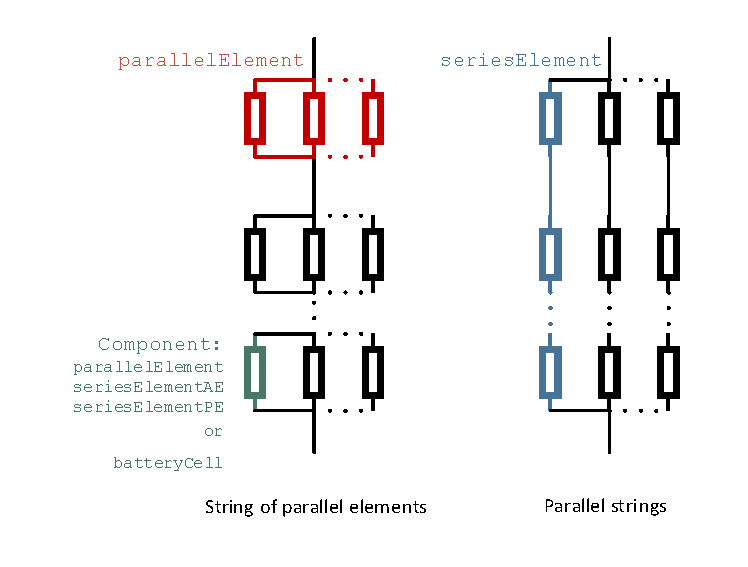
\includegraphics[width=\textwidth]{topologies2.pdf}
	\caption[Visualization of the possible battery topology compositions]{Visualization of the possible battery topology compositions.}
	\label{fig:topologies2}
\end{figure}
Figure~\ref{fig:topologies2} provides a visual overview of the topologies that are possible using different compositions. Using this variation of the Composite design pattern, the components can be combined in any possible way at runtime. The most common battery topologies are strings of parallel elements (SP) and parallel strings of cells (PS)~\cite{cordoba-arenas_control-oriented_2015}. In Figure~\ref{fig:topologies2}, these would be the case if the composition's leaf nodes (cells) were all in the second layer (marked green). However, since every component can be either a cell or another composite, more complicated topologies are made possible in this package. \\
\begin{figure}[t!]
	\captionsetup{type=figure}
	\centering
	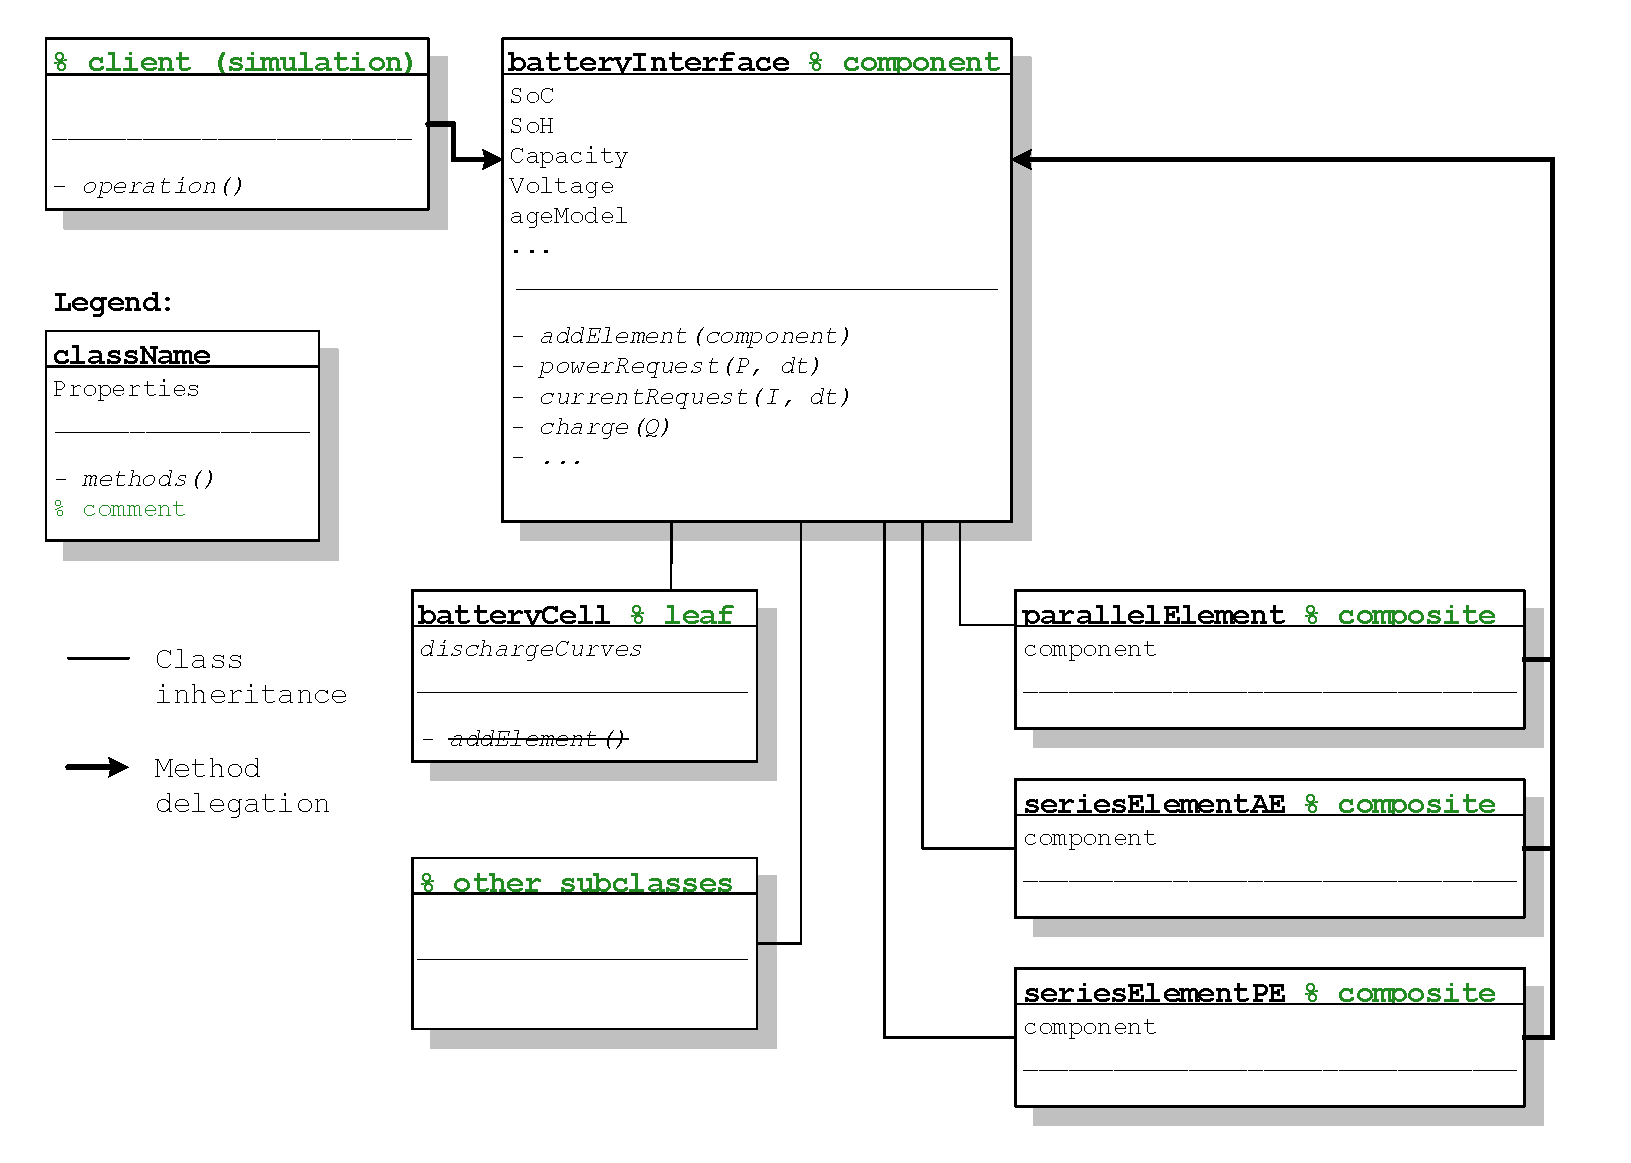
\includegraphics[width=\textwidth]{composite_schema.pdf}
	\caption[Class diagram of the battery composition with communication flows and inheritance links]{Class diagram of the battery composition with communication flows and inheritance links.}
	\label{fig:composite_schema}
\end{figure}

\subsection{Method delegation}
A pattern diagram of the classes used for the topology composition is depicted in Figure~\ref{fig:composite_schema}. Every composite element holds a reference to a component and delegates the methods called on it to said component. The delegated methods are wrapped with the rules of the respective topology in a similar fashion as is done with the Decorator design pattern. An example of the method delegation for a PS configuration - a \mcode{parallelElement} that holds a set of \mcode{seriesElement} objects, each in turn holding a set of \mcode{batteryCell} objects - is visualized in Figure~\ref{fig:method_delegation}. In this example, a current \mcode{I} and the simulation time step size is passed to the \mcode{parallelElement} via a \mcode{getVoltage()} method. The \mcode{parallelElement} determines which portion of \mcode{I} to send to each of it's components and delegates the method. Each \mcode{seriesElement} does the same and delegates the method to it's \mcode{batteryCell} objects. These return their voltages back to the \mcode{seriesElement} objects, which sum up the results received from their cells and pass the sum back to the \mcode{parallelElement}. Finally, the \mcode{parallelElement} calculates the mean of all the summed up voltages it received and passes the end-result back to the client.
\begin{figure}[t!]
	\captionsetup{type=figure}
	\centering
	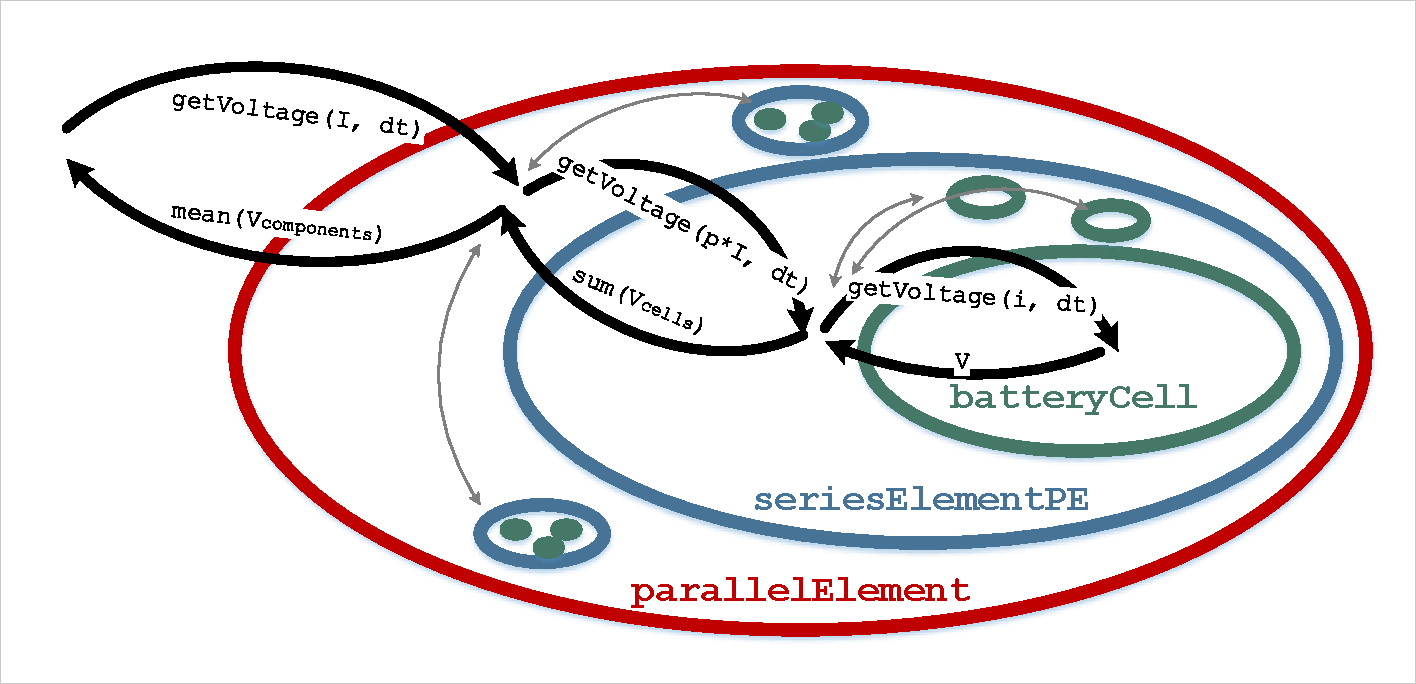
\includegraphics[width=\textwidth]{method_delegation.pdf}
	\caption[Example of a method being delegated across a battery pack composition]{Example of a method being delegated across a battery pack composition.}
	\label{fig:method_delegation}
\end{figure}
The following operations are delegated by an object that implements the \mcode{batteryInterface}:
\begin{itemize}
	\item Determination of the new voltage after charging or discharging a with a certain current and time step size. This is delegated to each \mcode{batteryCell} object's \mcode{dischargeCurves} reference.
	\item Charging or discharging the battery.
	\item Determining the state of the battery if it were to be charged or discharged.
	\item Determining the maximum charging or discharging current.
	\item Calculating the pack's $SoH$.
	\item Getters and setters for the component's voltage and capacity properties.
	\item Getter for the component's internal impedance. 
\end{itemize}
With the number of subcomponents $n$, a component's voltage is determined as
\begin{equation} 
V\subi{component} = \left\lbrace
\begin{smallmatrix}
\frac{\sum_{i=1}^{n}V\subs{subcomponent}{i}}{n} & \text{for a parallel element}\\
& \\
\sum_{i=1}^{n}V\subs{subcomponent}{i} & \text{for a series element} \\
\end{smallmatrix}
\right.
\end{equation}
And a component's capacity is
\begin{equation}
C\subi{component} = \left\lbrace
\begin{smallmatrix}
\sum_{i=1}^{n}C\subs{subcomponent}{i} & \text{for a parallel element}\\
& \\
\min_{i=1}^{n}C\subs{subcomponent}{i} & \text{for a series element with passive equalization} \\
& \\
\frac{\sum_{i=1}^{n}C\subs{subcomponent}{i}}{n} & \text{for a series element with active equalization}\\
\end{smallmatrix}
\right.
\end{equation}
Since the $SoH$ is derived directly from the capacity (see Equation~\ref{eq:age_soh}), a component's $SoH$ can be determined in the same fashion.
\begin{equation}
SoH\subi{component} = \left\lbrace
\begin{smallmatrix}
\sum_{i=1}^{n}SoH\subs{subcomponent}{i} & \text{for a parallel element}\\
& \\
\min_{i=1}^{n}SoH\subs{subcomponent}{i} & \text{for a series element with passive equalization} \\
& \\
\frac{\sum_{i=1}^{n}SoH\subs{subcomponent}{i}}{n} & \text{for a series element with active equalization}\\
\end{smallmatrix}
\right.
\end{equation}
Due to the fact that the model is based on curve fits, the internal impedance $Z\subi{i}$ property is not used for modelling the charging behaviour directly. It does however, determine how the voltages and currents are distributed across the subcomponents when charging or discharging. The impedance proportionality factor $p\subi{z}$ of a subcomponent with index $j$ is the component's $Z\subi{i}$ divided by the sum of all subcomponents' $Z\subi{i}$.
\begin{equation}
p\subs{z}{j} = \frac{Z\subs{i}{j}}{\sum_{i=1}^{n}Z\subs{i}{i}}
\end{equation}
When charging, a series element with active equalization will distribute it's voltage equally across all of it's subcomponents to account for balancing, while a series element with passive equalization will distribute it's voltage according to $p\subs{z}{j}$. For a parallel element, the current is distributed in such a way that the subcomponent $j$ with the lowest $Z\subi{i}$ receives the highest current.
\begin{equation}
I\subs{subcomponent}{j} = \frac{\frac{1}{p\subs{z}{j}}}{\sum_{i=1}^{n}\frac{1}{p\subs{z}{i}}}
\cdot I\subi{component}
\end{equation}


\subsection{Battery Interface}
The battery interface is described in the following subsections. Every component implements the \mcode{batteryInterface}, so the methods described in this section can be called on \mcode{batteryCell} objects and on the composites.

\subsubsection{Battery object initialization}
To initialize a battery object at runtime, the nominal capacity $C\subi{n}$ in Ah and the nominal voltage $V\subi{n}$ in V must be passed to a \mcode{batteryCell} constructor. A composite can be initialized as an "empty" circuit element and the cell (or other composites) can be added to it via it's \mcode{addElements()} method\footnote{Here, "empty" is referred to in the sense of not holding any cells, not in the sense of an empty \matlab\ variable.}.

\begin{lstlisting}
% Initialize an "empty" parallel element
bat = parallelElement;
Cn = 3; % Nominal cell capacity in Ah
Vn = 3.2; % Nominal cell voltage in V
% Initialize 3 battery cells and add them to bat
for i = 1:3
	b = batteryCell(Cn, Vn);
	bat.addElements(b);
end
\end{lstlisting}
The \mcode{addElements()} method also accepts component arrays...
\begin{lstlisting}
for i = 1:3
	b(i) = batteryCell(Cn, Vn);
end
bat.addElements(b);
\end{lstlisting}
...and multiple inputs:
\begin{lstlisting}
b1 = batteryCell(Cn, Vn);
b2 = batteryCell(Cn, Vn);
b3 = batteryCell(Cn, Vn);
bat.addElements(b1, b2, b3);
\end{lstlisting}
To create a composition like the example in Figure~\ref{fig:method_delegation} (see also Figure~\ref{fig:topologies2}, right), the following syntax could be used:
\begin{lstlisting}
% Initialize "empty" parallel element
bat = parallelElement;
% Initialize 3 "empty" series elements each holding 3 cells
for i = 1:3
	se = seriesElementPE; % passive equalization
	for j = 1:3
		se.addElements(batteryCell(Cn, Vn))
	end
	% Add series elements to bat
	bat.addElements(se)
end
% Further initialization operations, e.g. bat.addcurves() here...
\end{lstlisting}

\subsubsection{Battery charging and discharging}
Battery charging \footnote{Discharging will also be referred to as charging (with a negative current) in this documentation.} is handled by the methods \mcode{powerRequest()} and \mcode{currentRequest()}. Both functions are called in a similar manner. The syntax is as follows:
\begin{lstlisting}
[P, V, I] = bat.powerRequest(P, dt);
[P, V, I] = powerRequest(bat, P, dt); % equivalent
[P, V, I] = bat.currentRequest(I, dt);
[P, V, I] = currentRequest(b, I, dt); % equivalent
\end{lstlisting}
Where \mcode{P} is the requested power $P$ in W, \mcode{I} is the requested current $I$ in A and \mcode{dt} is the simulation time step size $\Delta t\subi{s}$ in s. The methods return the actual power throughput in W, the battery's voltage $V$ at the end of the time step and the actual current throughput in A. The returned power and current is limited by the $SoC$ or the cells' maximum currents, among other factors.
\begin{figure}[b!]
	\captionsetup{type=figure}
	\centering
	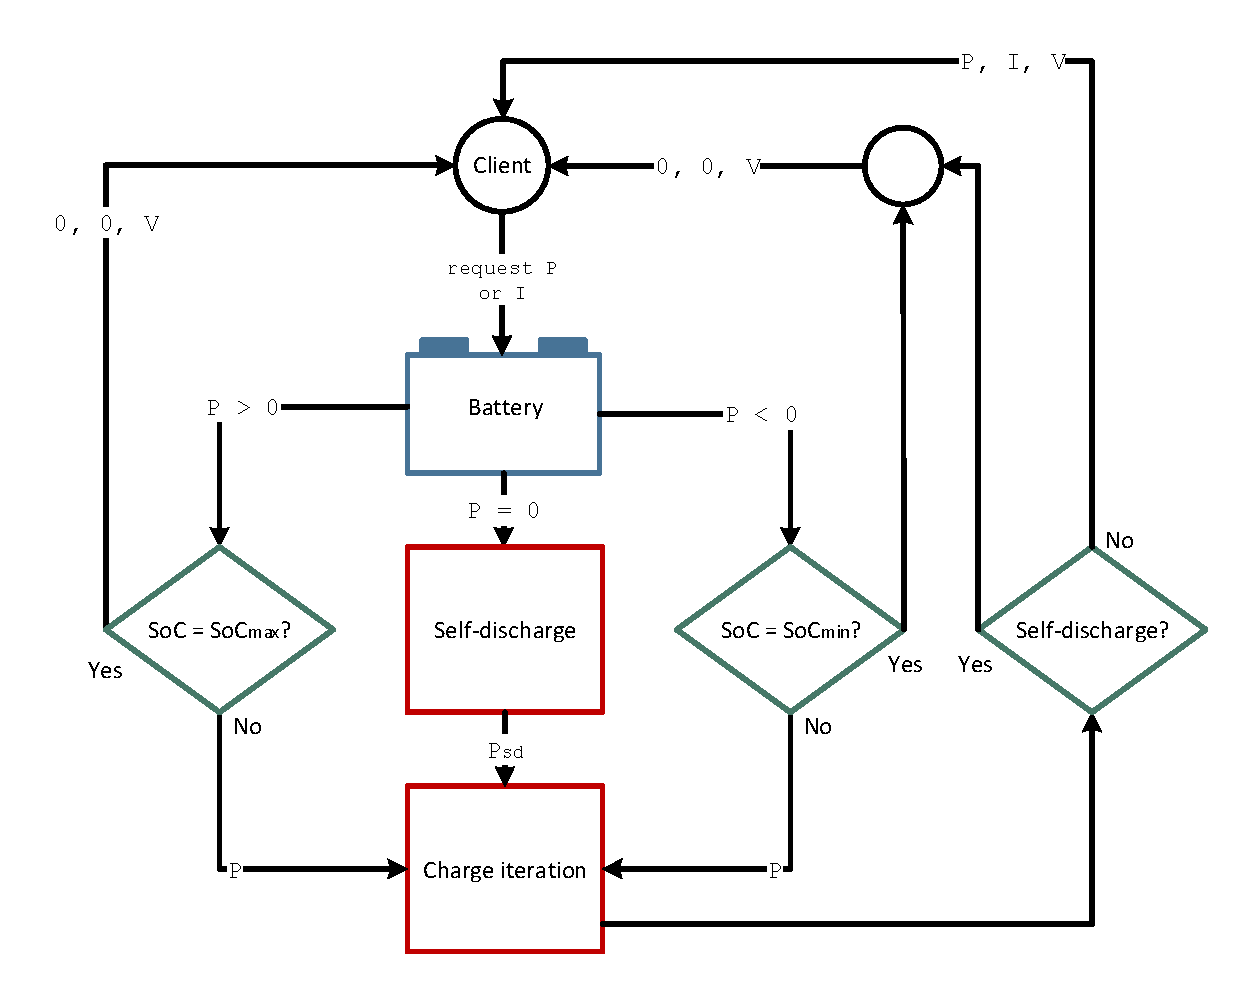
\includegraphics[width=\textwidth]{powerRequest.pdf}
	\caption[Flow chart of the \mcode{powerRequest()} and \mcode{currentRequest()} methods]{Flow chart of the \mcode{powerRequest()} and \mcode{currentRequest()} methods.}
	\label{fig:powerRequest}
\end{figure}
Figure~\ref{fig:powerRequest} contains a flow chart of the charging process. The client sends a request to the battery. If the requested power is not equal to zero and the battery's $SoC$ is not already at it's upper or lower limit, a charge iteration is performed (the \mcode{iteratePower()} and \mcode{iterateCurrent()} methods are called, respectively) and the resulting power, current and voltage are returned to the client. A positive input to the charge iteration  indicates charging and a negative input specifies discharging. If the request is zero, signalling that the battery is in an idle state, a logical flag is set to true and the charge iteration is called with the battery's self-discharge $P\subi{sd}$. The logical flag is checked after every call to the charge iteration methods in order to return a power and current of zero to the client if it was set to true. If the $SoC$ is either at it's upper or lower limit, the battery simply returns it's voltage along with a power and current of zero.\\
\begin{figure}[t!]
	\captionsetup{type=figure}
	\centering
	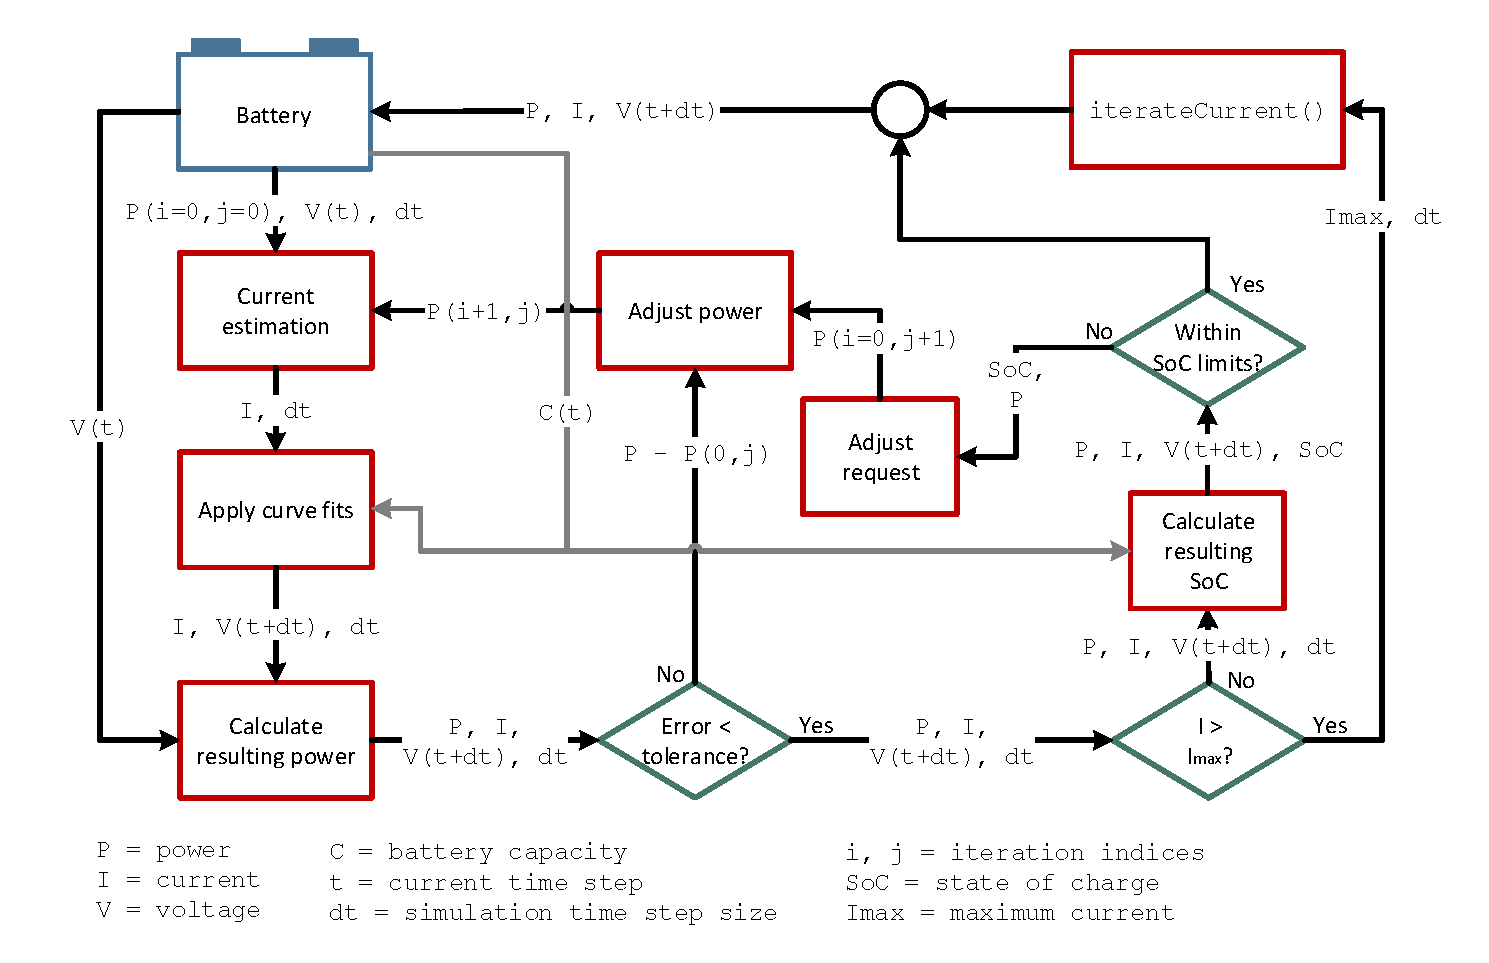
\includegraphics[width=\textwidth]{iteratePower.pdf}
	\caption[Flow chart of the \mcode{iteratePower()} method]{Flow chart of the \mcode{iteratePower()} method.}
	\label{fig:iteratePower}
\end{figure}
A flow chart of the \mcode{iteratePower()} method is depicted in Figure~\ref{fig:iteratePower}. First, a current is estimated from the requested power and the battery's voltage. The current and the time step size are then delegated to the battery cells' \mcode{dischargeCurves} objects, in order to determine the resulting voltage. An approximation of the power is determined from the mean of the returned voltage and the battery's old voltage. This is repeated through recursion until the difference between the iterated power and the originally requested power meets a certain tolerance. If the resulting current is greater than the battery's maximum current $I\subi{max}$, the \mcode{iterateCurrent()} method is called using $I\subi{max}$ as an input. It's output current, the resulting power and voltage are returned. Otherwise, the $SoC$ is determined and compared the battery's upper and lower limit. If the $SoC$ is within the interval $[SoC\subi{min}, SoC\subi{max}]$, the power, current and voltage are returned. Otherwise, the requested power is adjusted according to the difference between the $SoC$ and the respective limit that was exceeded, thus starting the iteration again. \\
\begin{figure}[t!]
	\captionsetup{type=figure}
	\centering
	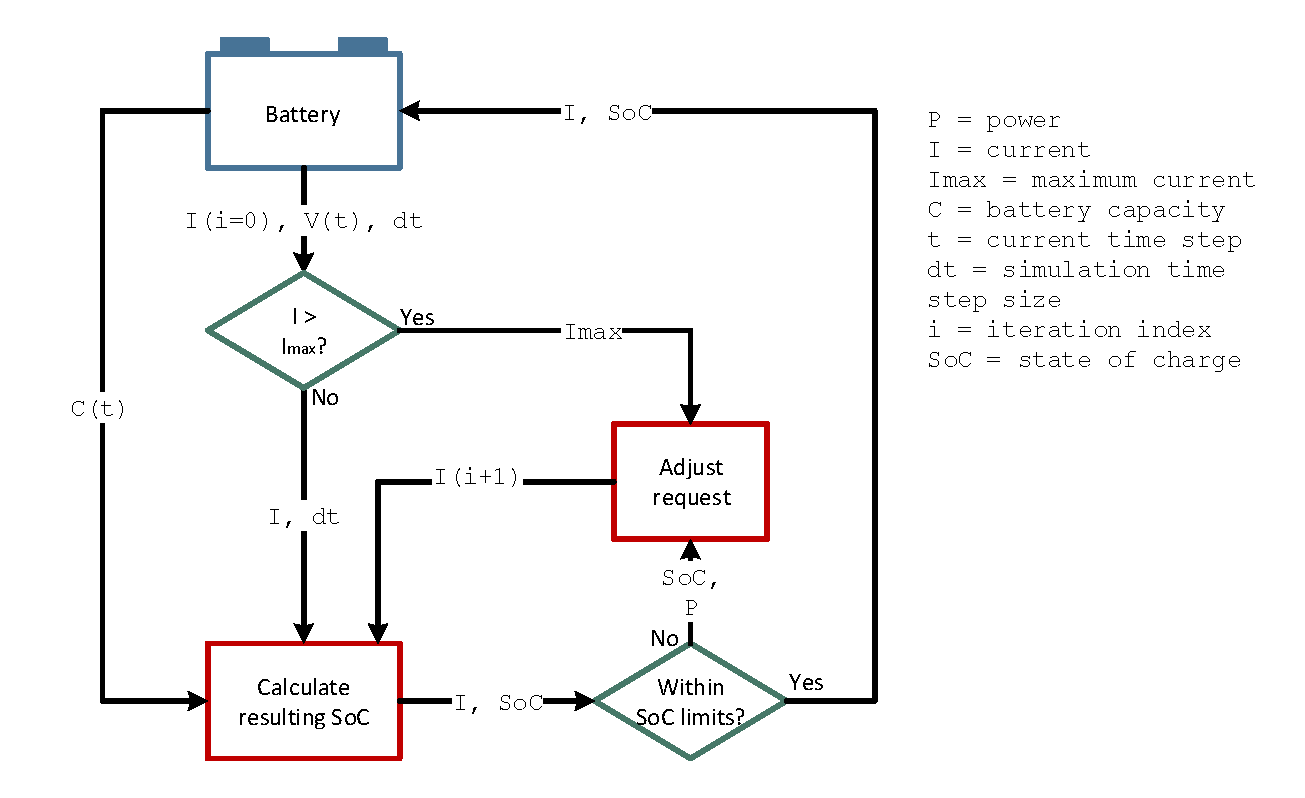
\includegraphics[width=\textwidth]{iterateCurrent.pdf}
	\caption[Flow chart of the \mcode{iterateCurrent()} method]{Flow chart of the \mcode{iterateCurrent()} method.}
	\label{fig:iterateCurrent}
\end{figure}
Figure~\ref{fig:iterateCurrent} depicts a flow chart of the \mcode{iterateCurrent()} function. Using this method is a lot faster than using the \mcode{iteratePower()} function, due to it's comparative simplicity. However, the current may need to be determined separately in some cases. Before the iteration, the current is limited to $I\subi{max}$. Finally, the another limitation is performed if the $SoC$ is not within the interval $[SoC\subi{min}, SoC\subi{max}]$. Normally, one or two iterations should suffice for returning the current and $SoC$. The voltage and power are not calculated and must be determined by calling the \mcode{getNewVoltage()} method if required\footnote{For example, this is done within the \mcode{currentRequest()} method, which does return the voltage and power.}.
%TODO: iteratePower() description
%TODO: iterateCurrent() description
%TODO: Figure showing "jumps" in the voltage with variable charging currents
\subsubsection{Age model level}